\subsection{WCA Lamp Images (aka, Lamp Family Portraits) \label{subsec:fportrait} }
\normalsize

The four panels of Figures~\ref{fig:FG21}--\ref{fig:FG24} show a `family portrait' of the available COS PtNe Lamp (\plampone{} or \plamptwo{}) + MIRROR (MIRA or MIRB)
combinations possible with \tacq{IMAGE}.
Panel titles give the lamp and mirror configuraton, along with the lamp current setting (in milli-amps, mA) and the exposure times.
The images and subarrays are in `detector' coordinates, as used on-board COS.
The images show the observed counts/pixel/s (cps) as given by the colorbar on the bottom.
The \textcolor{red}{red} dashed boxes show the given cycles' \tacq{IMAGE} WCA subarrays. At the top of the subarrays, text provides the count rate in the brightest pixel (BP) in units of cps.
The \textcolor{blue}{blue} histogram on the bottom edge shows the cross-dispersion (XD) lamp profile in detector `X$_{DET}$' coordinates, while
the \textcolor{green}{green} histogram on the left edge shows the along-dispersion (AD) lamp profile in detector `Y$_{DET}$' coordinates.
The cross-hairs show the median location of the given configurations' lamp events within the TA subarray.
PtNe\#2 (\plamptwo{}) lamp was used for all \tacq{IMAGE}s during C20--24, and was operated at LOW current (6~mA) for MIRA images
and LOW current (3~mA) or MEDium current (10~mA) for the MIRB, depending on the Cycle. Note the separate MIRB images in about a 2:1 ratio, and the asymmetric
(toward -XD) scattered light.

See the figure captions for specific details about each cycles' family portrait.

\begin{figure}[htb]
\noindent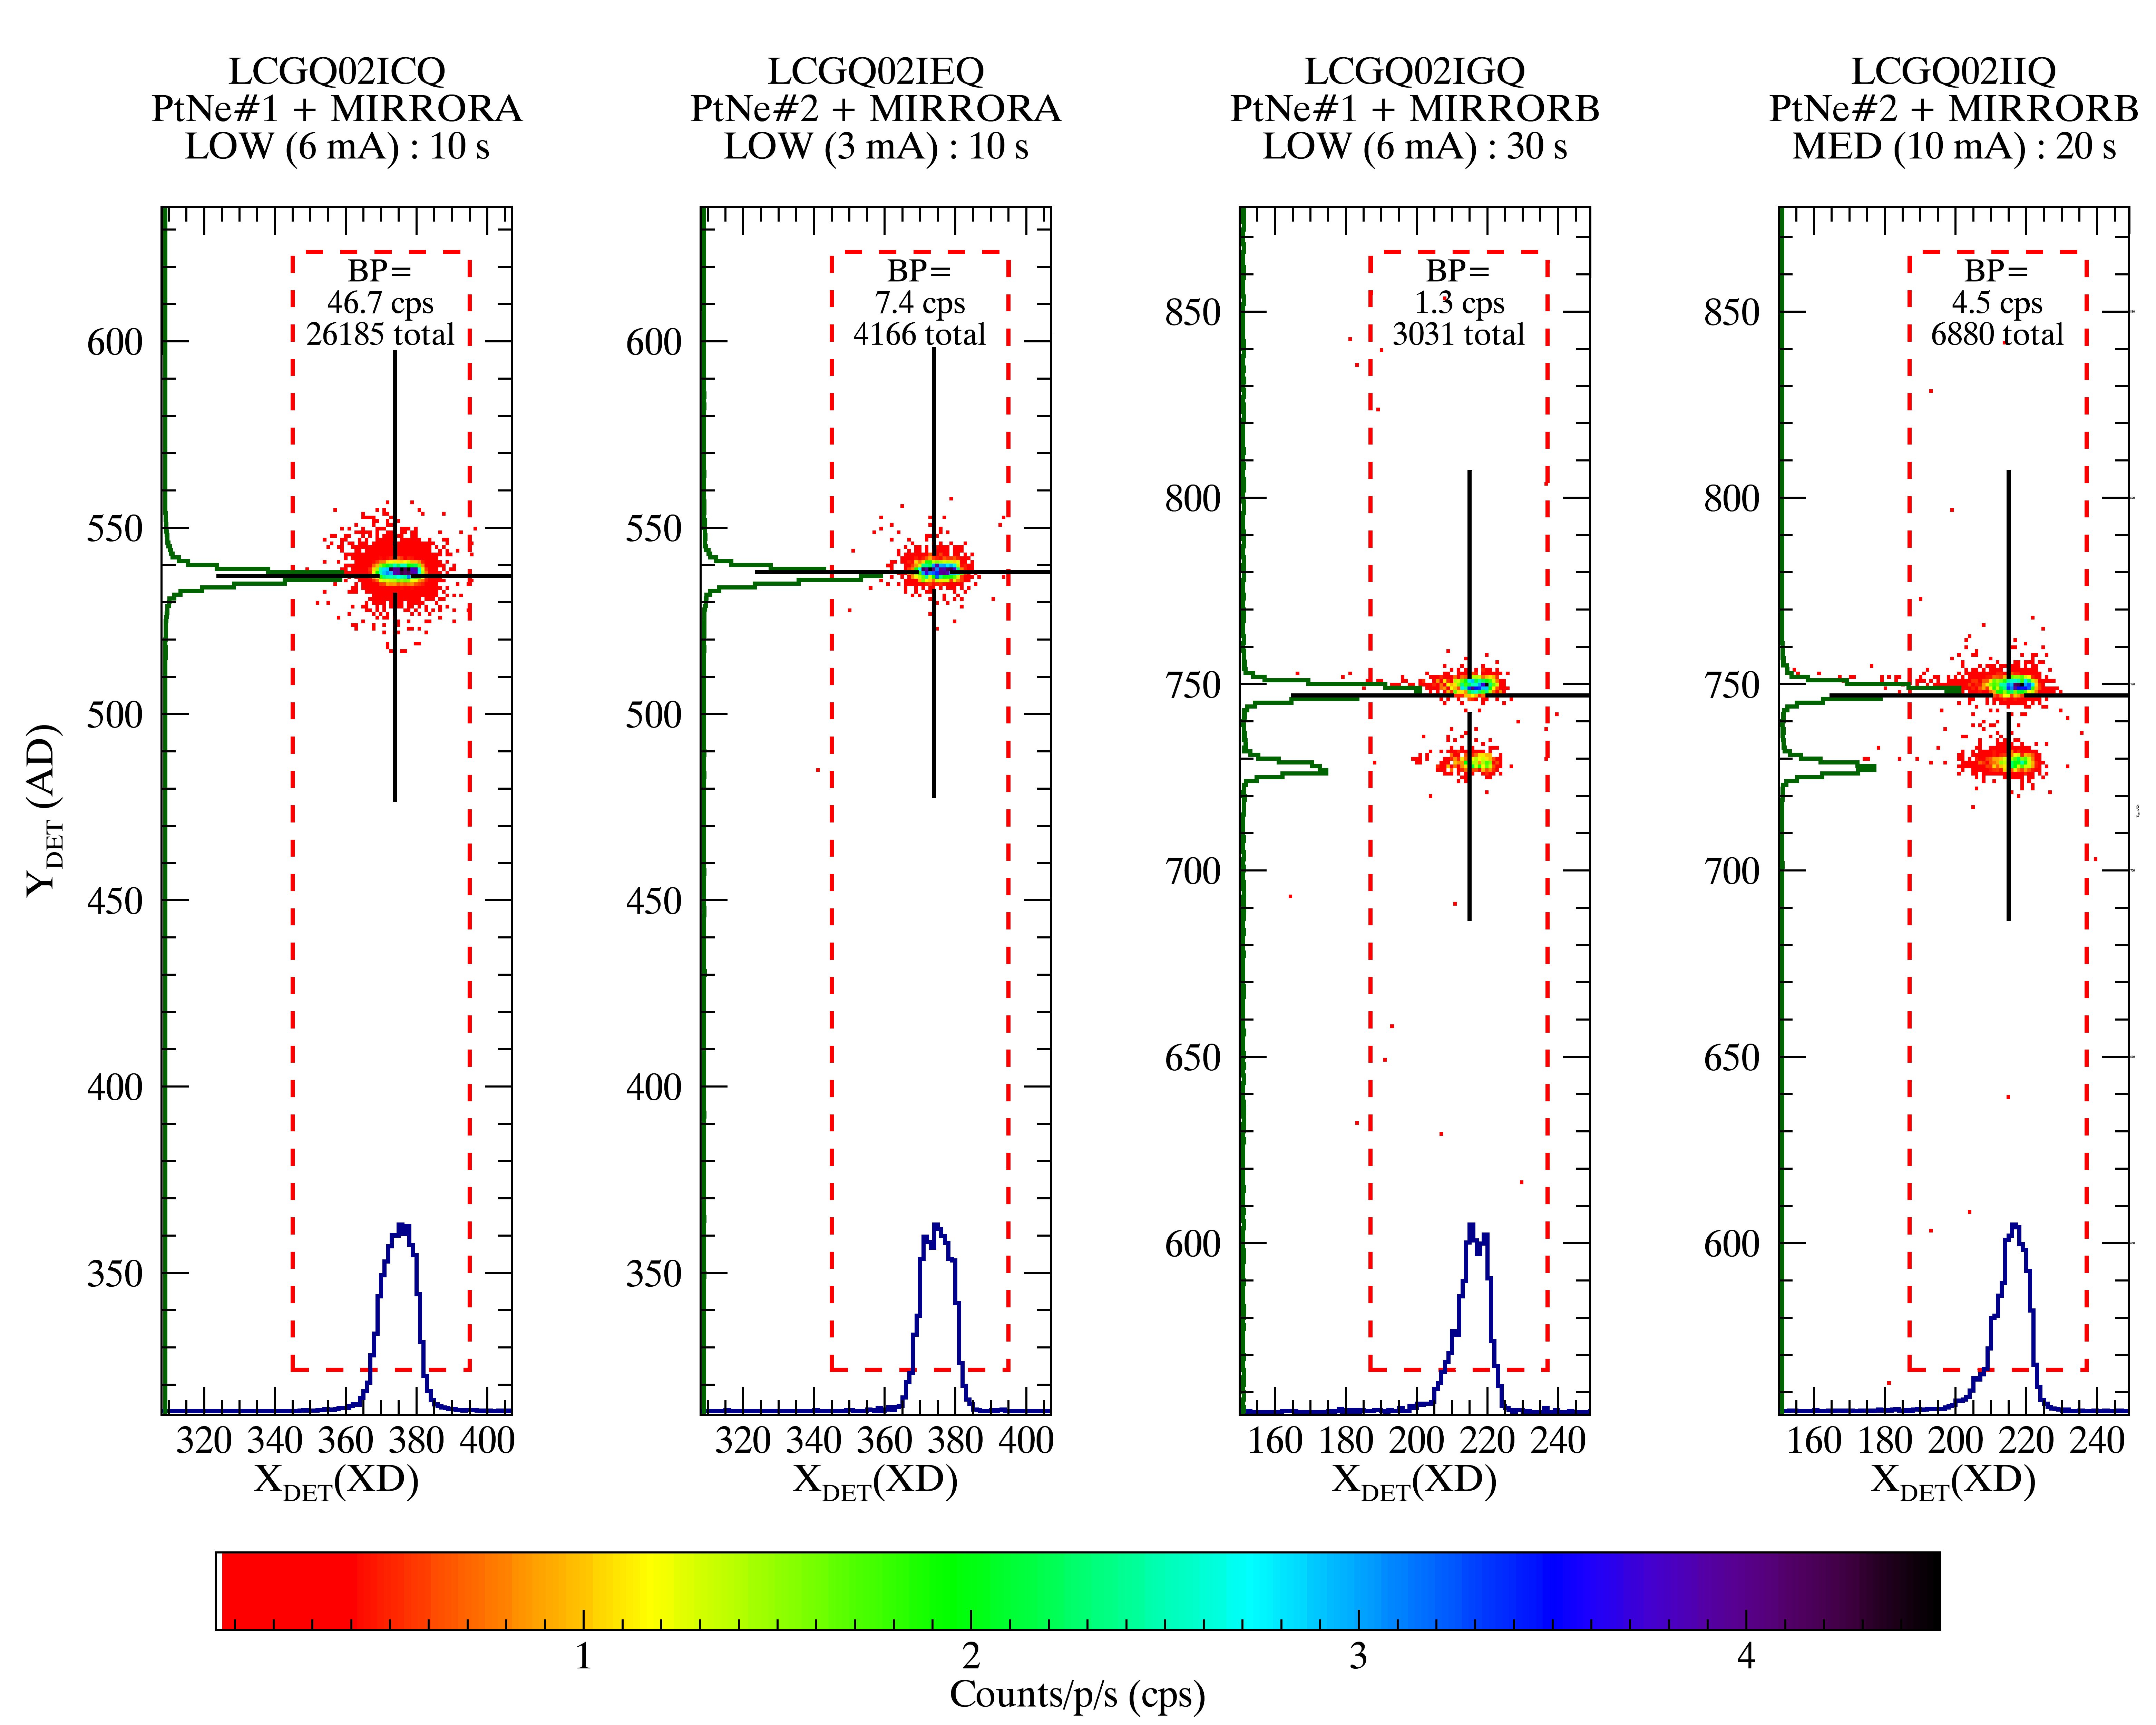
\includegraphics[width=1.0\linewidth]{png/C21_13526_FP.png}
\caption[C21 WCA Lamp `Family Portrait']{Cycle~21 (\pid{13526} PtNe Lamp `Family Portrait'
counts per second per pixel (cps) NUV images of the internal PtNe lamps (\plampone{} \& \plamptwo{}) through the
WCA using either MIRRORA (MIRA, left 2 panels) or MIRRORB (MIRB, right 2 panels). The titles
give the exposure \textit{ROOTNAME}, configuration, exposure time and lamp current. Cross hairs show median locations and dashed
lines show the \textsc{LTAIMCAL} TA subarrays.
The insert text gives the Brightest Pixel (BP) in cps and the total counts in the subarray.
AD and XD profiles are given along each axis, and the color bar at the
bottom applies to all four images. Note the separate MIRB images in about a 2:1 ratio, and the asymmetric
(toward -XD) profile and scattered light. All panels are in detector (DET) coordinates.\label{fig:FG21}}
\end{figure}
\begin{center}
	\begin{figure}[htb]
	\noindent\includegraphics*[width=1.0\linewidth]{png/C22_13972_FP.png}
	\caption[C22 WCA Lamp `Family Portrait']{\footnotesize Cycle~22 PtNe Lamp `Family Portrait' (see Fig~\ref{fig:FG21}).
	Note that during both the MIRA and MIRB images, the lamp image is about -50~p from the C21 AD location (Y$_{DET}$).
	This is common, and the TA subarrays must be large enough to account for this offset.\label{fig:FG22}}
	\end{figure}
\end{center}
\begin{center}
\begin{figure}[htb]
\noindent\includegraphics*[width=1.0\linewidth]{png/C23_14440_FP.png}
\caption[C23 WCA Lamp `Family Portrait']{Cycle~23 PtNe Lamp `Family Portrait' (see Fig~\ref{fig:FG21} \& Fig~\ref{fig:FG22}).
	Note that during all images, the lamp image is about +50~p from the C22 AD location (Y$_{DET}$),
	and has returned to its C21 AD position.\label{fig:FG23}}
\end{figure}
\end{center}
\begin{center}
	\begin{figure}[htb]
	\noindent\includegraphics*[width=1.0\linewidth]{png/C24_14857_FP.png}
	\caption[C24 WCA Lamp `Family Portrait']{Cycle~24 PtNe Lamp `Family Portrait' (see Fig~\ref{fig:FG21}--Fig~\ref{fig:FG23}).
	Note that during all images, the lamp image has returned to its C21 position.\label{fig:FG24}}
	\end{figure}
\end{center}
